\documentclass[../main.tex]{subfiles}
\graphicspath{
    {"../img/"}
    {"img/"}
}
\begin{document}

\subsection{funkcje wielu zmiennych}

\begin{przyklad}
    \begin{align*}
        &\mathbb{R}^{3}\rightarrow\mathbb{R}^{1} \text{ - Energia potencjalna } \mathcal{V}(x,y,z)\\
        &\mathbb{R}^{4}\rightarrow\mathbb{R}^{1} \text{ - Potencjał pola niestacjonarnego} \mathcal{V}(x,y,z,t)\\
        &\mathbb{R}^{3}\rightarrow\mathbb{R}^{3} \text{ - Natężenie pola } \mathcal{E}(x,y,z) \\
        &\mathbb{R}^{4}\rightarrow\mathbb{R}^{3}\\
        &\mathbb{R}^{1}\rightarrow\mathbb{R}^{3}\\
        &\mathbb{R}^{1}\rightarrow\mathbb{R}^{4}\\
        &\mathbb{R}^{1}\rightarrow\mathbb{R}^{6}\\
        &\mathbb{R}^{6}\rightarrow\mathbb{R}^{1}\\
        &\mathbb{R}^{8}\rightarrow\mathbb{R}^{1}\\
    .\end{align*}
\end{przyklad}

\begin{definicja}
    (Ciągłość Heine)\\
Niech $X\subset\mathbb{R}^n, x_{0} \in X, Y\subset\mathbb{R}^m$. Mówimy, że odwzorowanie $T: X\rightarrow Y$ jest ciągłe w punkcie $x_0$, jeżeli $$\underset{x_n \to x_0}{\forall}, T(x_{n})\rightarrow T(x_{0})$$\\
    \textbf{Uwaga: } $x_{0} = (x_{1}, x_{2}, ..., x_{n})$.
\end{definicja}

\begin{pytanie}
    Czy ciągłość w $\mathbb{R}^{n} \iff$ ciągłośc w $\mathbb{R}^{1}$?
\end{pytanie}

\begin{przyklad}
    Niech funkcja

\[ f(x,y) =
\begin{cases}
    0                           & \quad x=y\\
    \frac{xy^2}{x^2+y^4}  & \quad x\neq y
\end{cases}
\]

czy $f$ - ciągła w $(0,0)$?
dla trajektorii I:

$$\lim\limits_{y_{n}\to 0}(\lim\limits_{x_{n}\rightarrow 0} f(x_{n},y_{n})) = \lim\limits_{y_{n}\rightarrow 0}(0) = 0$$

dla trajektorii II:

$$\lim\limits_{x_{n}\to 0}(\lim\limits_{y_{n}\rightarrow 0} f(x_{n},y_{n})) = \lim\limits_{x_{n}\rightarrow 0}(0) = 0$$

weźmy $(x_{n},y_{n}) = (\frac{1}{n^{2}},\frac{1}{n})$

$$f(x_{n},y_{n}) = \frac{\frac{1}{n^{2}} \frac{1}{n^{2}}}{\frac{1}{n^{4}}+\frac{1}{n^{4}}} = \frac{1}{2} \neq \lim\limits_{x_{n}\to 0, y_{n}\to 0} f(0,0)$$
\end{przyklad}

\begin{figure}
    \centering
    \begin{center}
        \includegraphics[width=0.48\textwidth]{fig_1}
    \end{center}
    \caption{trajektoria I i II}
\end{figure}


\begin{definicja}
    (Ciągłość Cauchy)\\
$(X,d_{X})$ - przestrzeń wektorowa z metryką $d_{X},\\ (Y,d_{Y})$ - p.w. z metryką $d_{Y}$.\\
Niech $x_{0}\in X$. Mówimy, że $T: X\to Y$ - ciągłe, jeżeli
$$\underset{\varepsilon > 0}{\forall} \quad\underset{\delta}{\exists} \quad\underset{x\in X}{\forall} d_{X} (x,x_{0}) < \delta \implies d_{Y} (T(x_{0}), T(x)) < \varepsilon$$
\end{definicja}

\begin{proof}
    Heine $\iff$ Cauchy

    \[\implies_{(\text{przez sprzeczność})}\]

Zakładamy, że
    \[
        \underset{x_n \to x_0}{\forall} T(x_{n}) \to T(x_{0})
    \]
    oraz
    \begin{equation}
        \label{eq:p_1.1}
        \underset{\varepsilon > 0}{\exists}, \underset{\delta > 0}{\forall}, \underset{x\in X}{\exists} : d_{X} (x,x_{0}) < \delta \quad\land\quad d_{Y} (T(x),T(x_{0})) \geq \varepsilon
    \end{equation}

Skoro $T(x_{n})\to T(x_{0}) \underset{x_n \to x_0}{\forall}$, to w szczególności warunek spełniony dla ciągu, który jest taki:

    Skoro (\ref{eq:p_1.1}), to dla $\varepsilon>0$ weźmy $\delta = 1$,

\begin{align*}
    &\delta=1:\\
    &&\underset{x_1}{\exists} \quad d_{X} (x_{1},x_{0})<1 \land d_{Y} (T(x_{1}), T(x_{0})) \geq \varepsilon \\
    &\delta=\frac{1}{2}:\\
    &&\underset{x_2}{\exists} \quad d_{X} (x_{2},x_{0})<\frac{1}{2} \land d_{Y} (T(x_{2}), T(x_{0})) \geq \varepsilon \\
    &\delta=\frac{1}{3}:\\
    &&\underset{x_3}{\exists} \quad d_{X} (x_{3},x_{0})<\frac{1}{3} \land d_{Y} (T(x_{3}), T(x_{0})) \geq \varepsilon\\
    &\vdots &\vdots\\
    &\delta=\frac{1}{n}:\\
    &&\underset{x_n}{\exists} \quad d_{X}(x_{n},x_{0}) < \frac{1}{n} \land d_{Y} (T(x_{n}),T(x_{0})) \geq \varepsilon
.\end{align*}

Zauważmy, że taki ciąg $x_{n} \to x_{0}$, ale $T(x_{n}) \not\rightarrow T(x_{0})$, więc mamy sprzeczność. $\Box$

    $\impliedby$ Wiemy, że
    \begin{equation}
        \label{eq:p_1.2}
        \underset{x_n\to x_0}{\forall}\quad \underset{\varepsilon > 0}{\forall}\quad \underset{x}{\exists}\quad d_{X} (x,x_{0}) < \delta \implies d_{Y} (T(x),T(x_{0})) < \varepsilon
    ,
    \end{equation}
czyli:

\begin{equation}
    \label{eq:p_1.3}
    \underset{\delta_1}{\forall} \quad\underset{N}{\exists} \quad\underset{n>N}{\forall} \quad d_{X} (x_{n}, x_{0}) < \delta_{1}
\end{equation}

Chcemy pokazać, że $T(x_n) \to T(x_0)$, czyli, że
    \[
        \underset{\varepsilon_1 > 0}{\forall} \underset{N_1}{\exists} \underset{n>N_1}{\forall} \quad d_Y (T(x_n),T(x_0)) < \varepsilon_1 (\text{dla } x_n \to x_0)
    \]

    Przyjmijmy $\varepsilon=\varepsilon_1$. Oznacza to, że $\underset{\delta}{\exists}$ spełniająca warunek (\ref{eq:p_1.2}) dla $\varepsilon_1$. Połóżmy $\delta_1=\delta$ we wzorze (\ref{eq:p_1.3}), czyli wiemy, że
    \[
        \underset{N}{\exists} \underset{n>N}{\forall} \quad d_X(x_n, x_0) < \delta_1,
    \]
    ale na mocy (\ref{eq:p_1.2}), wiemy, że
    \[
        d_Y (T(x_n),T(x_0)) < \varepsilon_1
    \]
\end{proof}

\pagebreak
\subsection{
    Różniczkowalność:
}

\begin{definicja}
    Pochodna cząstkowa:\\
    Niech $\mathcal{O}\subset\mathbb{R}^{n}, \mathcal{O}$ - otwarty,
    $f: \mathcal{O}\to\mathbb{R}^{1}, x\in\mathbb{Q}, x_0 = (x_1^0,x_2^0,\dots,x_n^0)$.\\
    Mówimy, że $f$ ma w punkcie $x$ pochodną cząstkową w kierunku $x^k$, jeżeli istnieje granica
    \[
        g \overset{\text{def}}{=} \lim\limits_{h \to 0}\frac{f(x_1^0, x_2^0, \dots, x_k^0 + h, \dots, x_n^0) - f(x_1^0,\dots,x_n^0)}{h} \equiv \left. \frac{\partial}{\partial x} f \right |_{x=x_0}
    \]
\end{definicja}

\begin{figure}
    \centering
    \includegraphics[width=0.8\textwidth]{fig_2}
    \caption{Problemy: Umiemy tak jak po lewej, ale nic nie potrafimy zrobić z tym po prawej}
    \label{fig:fig_2}
\end{figure}

\begin{przyklad}
    Pochodna cząstkowa\\

    Niech $\mathbb{R}^{2}\to\mathbb{R}^{1}$.
    \begin{align*}
        &\frac{\partial}{\partial x} f = \lim\limits_{h \to 0}\frac{f(x+h,y) - f(x,y)}{h},\\
        &\frac{\partial}{\partial y} f = \lim\limits_{h \to 0}\frac{f(x,y+h) - f(x,y)}{h}
    .\end{align*}

    \textbf{Uwaga:} do policzenia pochodnej czątkowej potrzebujemy układu współrzędnych.
    \[
        \text{biegunowy } \to f(r,\varphi)
    .\]
\begin{align*}
    &\frac{\partial f}{\partial r} = \lim_{h \to 0} \frac{f(r+h, \varphi) - f(r,\varphi)}{h}\\
    &\frac{\partial f}{\partial \varphi} = \lim_{h \to 0} \frac{f(r, \varphi + h) - f(r,\varphi)}{h}
.\end{align*}

\end{przyklad}

\pagebreak
\begin{definicja}
    Pochodna kierunkowa:\\
    Niech $\mathcal{O}\subset\mathbb{R}^{n}$, $\mathcal{O}$ - otwarte, $x_0\in\mathcal{O},e\in\mathcal{O},T:\mathcal{O}\to\mathbb{R}$.\\
    Mówimy, że $T$ ma w $x_0$ pochodną kierunkową (\textit{spoiler:} pochodną słabą), jeżeli istnieje granica
    \[
        g = \lim\limits_{t \to 0}\frac{T(x_0 +te) - T(x_0)}{t} \equiv \nabla_e T(x_0)
    .\]
\end{definicja}

\textbf{Obserwacja:} Jeżeli np.
$T: \mathbb{R}^{2}\to\mathbb{R}, e_x=(1,0)= \begin{bmatrix} 1\\0 \end{bmatrix} $ i $e_y = (0,1) = \begin{bmatrix} 0\\1 \end{bmatrix} $, to
\[
    \nabla_{e_{x}} T = \frac{\partial}{\partial x} T \text{ i } \nabla_{e_{y}} T = \frac{\partial}{\partial y} T
.\]

\begin{przyklad}
    Problemy z pochodną kierunkową:\\

$f(x,y) = \sqrt{|xy|}$. Wówczas $x_0 + te = (0+t1,0)$, $x_0 = (0,0), e_x = \begin{bmatrix} 1\\0 \end{bmatrix} $

    \[
        \left. \nabla_{e_x} f \right|_{x=(0,0)} = \lim\limits_{t \to 0}\frac{f(0+t,0) - f(0,0)}{t} = \lim\limits_{t \to 0}\frac{\sqrt{|t \cdot  0|} - \sqrt{|0 \cdot 0|}}{t} = \lim\limits_{t \to 0}\frac{0}{t} = 0 = \left. \frac{\partial}{\partial x} f\right |_{(0,0)}
    \]

\textbf{Uwaga:} $f(x) = \sqrt{x}, \mathbb{R}\to\mathbb{R}, f'(0) = \lim\limits_{h \to 0}\frac{\sqrt{h}}{h} = \pm \infty$

\[
f(x,y) =
    \begin{cases}
        0 & \quad x=y\\
        \frac{xy^2}{x^2+y^4} & \quad x \neq y\\
    \end{cases}
\]

$e = \begin{bmatrix} h_1\\h_2 \end{bmatrix}$. Pochodna: $\left. \nabla_e f\right |_{x=(0,0)}, (x_0 + te = (th_1, th_2))$

$$\lim\limits_{t \to 0}\frac{f(th_1, th_2) - f(0,0)}{t} = \frac{h_1 h_2^2}{h_1^2} = \frac{h_2^2}{h_1}$$
\end{przyklad}

\end{document}
